\chapter{Discussion}
\label{Discussion}
This section presents an analysis and discussion of the results. 

\section{Graph Behavior}
\Cref{tab:results:graph_behavior} presents illustrative examples rather than a comprehensive analysis. 
The behaviors shown represent typical trends observed when varying each parameter in the specified direction, but they may not apply to all possible values or reflect the magnitude of changes. 
Additionally, these results do not necessarily generalize to scenarios where two parameters are simultaneously varied. 
\Cref{tab:results:graph_behavior} should be interpreted alongside the local $S1$ sensitivities from \nameref{sec:SOBOL_sensitivity_analysis_results} to better understand how sensitive the output is to specific parameters and the potential impact of their variation.

\section{A Good Curve}
As the bacterial population grows, resource consumption accelerates until only trace amounts remain at $t=8$. 
The delay between the peaks of uninfected and infected bacteria is due to the infection stages and the latent period of phage infection. 
Each bacterium progresses from infection stage $k$ to $k+1$ at a rate of $\frac{M}{\tau}$. 
Therefore, decreasing the number of infection steps $M$ or increasing the latent period $\tau$ amplifies this delay. 
A longer latent period means it takes more time for bacteria to progress through the infection stages.

At $t=4$, the infection rate surpasses the bacterial replication rate, causing the bacterial population to decline even though resources are still available. 
This moment coincides with the rise of the phage population. 
Observing the timing of these events and changes in graph behavior, as well as their relationships across different graphs, helps clarify the complex population dynamics and the interdependence of the populations that might not be obvious from reading the ODE model. 

This becomes more difficult when the model goes from a $1\times1\times1$ system to a $p\times b \times r$ system. 
Now up to any number of phages can interact with any number of bacteria, and any number of bacteria can interact with any number of resources at varying rates. 
These varying rates will significantly influence the dynamics of the system, and make it hard to determine what event caused what due to the rise in number of interactions.
For a $1\times1\times1$ system, there are 2 interactions that can occur (assuming no self interactions, and that phages don\t interact with the resources). 
With a $p\times b\times r$ system, there are $\mathcal{O}(p\cdot b + b\cdot r)$ interactions that can occur. 
So for a $3\times2\times3$ system, there are at most 12 interactions occurring. 
12 events can occur at the same time, making it hard to identify the cause of the event. 

\section{SOBOL Sensitivity}
SOBOL, when mixed with a qualitative analysis can provide insight into why when a parameter changes, the output changes as it does. 
A mathematician or biologist might look at an ODE model and reason through the changes. 
They might explore the model by having an internal monologue as follows. 
“If I increase $\tau$, which means that the bacteria infection process takes longer, then when a phage infects a bacterium, it will take longer for the bacteria to die. 
Dying later means that the phages are released later. 
By releasing later, it will take longer for the phages to grow and peak. 
It also allows more time for the uninfected bacteria population to grow and use up the resources. 
There will be a natural delay in uninfected bacteria peak as it takes longer for the bacteria to become infected and go through the infection process.”
\Cref{tab:results:graph_behavior} aims to do this, but summarized to just the end result. 
However, these changes can't always be (accurately) quantified, without access to a graph of the simulation. 
Trying to accurately quantify these changes for multiple parameters takes time, and trying to reason through changing two or more parameters at a time is hard. 

A data scientist or modeler might use SOBOL to quantify these changes, and use the analysis from the biologist to gain a better oversight. 
The data scientist would be able to understand if the change in output value occurred because of that specific parameter of if it is a combination of parameters. 
The data scientist might not know if changing $\tau$ would result in more or less bacteria, but they would know that $\tau$ has an important role for the total bacteria population, but less so for resources. 
Then using the biologist's interpretation, they can piece together that changing $\tau$ to a larger number wont affect the resource cosnumption much, but that the bacteria population will show a significant increase in bacteria population. 

\subsection{Final Value Analysis}
\subsubsection{Resources}
For most simulations, all resources no matter the initial value, will have been used up before the end of the simulation. 
So on average, the final value for resources will be 0. 
This explains why the resource sensitivity is so high. 
There are some combinations of parameters that when chosen, will result in not all the resources being used up. 
For example, with \Cref{tab:appendixE:a_good_curve_2}, if $r=0.2$, not all the resources have been used up. 
Every parameter affects how the bacteria and phage population grows in some way, which influences the consumption rate of resources, which determines the final resource value. 
Of the other parameters, $\tau$ has the biggest influence because $\tau$ determines how fast the bacteria will go through the infection process. 
The longer it takes, the longer it takes for the phage population to grow, allowing more bacteria to grow and consume resources. 

\subsubsection{Phages}
The $r$ value allows the phages to infect the uninfected bacteria. 
$r$, the adsorption rate of phages to bacteria, can be interpreted as the efficiency of infection. 
The smaller the value, the more efficient the infection process is, and fewer phages it requires to infect a bacterium. 
With a larger $r$ value, more phages are used to infect a bacterium. 
$\beta$ has an influence on the final phage population, as the infected bacterium will release $\beta$ phages into the system. 
The more phages that are created for every lysed bacterium, the more phages are available in the system. 
But larger $r$ values will effectively require more phages to infect the bacterium. 

\subsubsection{Total Bacteria}
Resources, $\tau$, $e$, and $\beta$ all play a critical role in the final population value of bacteria. 
More resources allow bacteria to grow for a longer time, allowing more bacteria to be created. 
$\tau$ determines the infection process. 
The larger $\tau$ is, the longer it takes for the bacteria to lyse and create new phages to infect other bacteria. 
$\beta$ has a very important role in determining the final bacteria population, but surprisingly $r$ has no role in determining the final bacteria population. 
$e$ determines how fast the resources are consumed. 
The larger $e$ is, the faster the resources are being consumed and depleted. 
So by lowering $e$, more bacteria will be created, and the time at which the bacteria peak at occurs later in time. 
Of course as $\beta$ changes value, it will have a large influence on the final bacteria population. 
More phages will cause more infections, slowing the spread of bacteria. 
However, $r$ surprisingly does not have an influence on the final bacteria population level. 


\subsection{Peak Value Analysis}
\subsubsection{Resources}
The peak value for resources in always starts at $t=0$ and is either decreasing or constant, never increasing in concentration. 
As SOBOL measures the change in initial resource concentration and the resulting max value reached, it associates the initial condition with the peak value. 

\subsubsection{Phages}
The barplot values for the peak value for phages using the 95\% rule has the same values as in the final value plot for the phages. 
This makes sense as there is no removal of phages from the system, so any phages created by $r$ or $\beta$ will stay in the system. 
As the population is ever-increasing, the final and peak value will be occurring near one another and are tightly associated with one another. 

\subsubsection{Total Bacteria}
The total bacteria peak population is much more sensitive to the different parameter values. 
The bacteria act as a link between the phages and resources. Any changes in the resource consumption rate or initial condition will affect the bacteria population. 
Likewise, any change in phage adsorption rate will affect the bacteria growth, which in turn will affect the resource consumption rate. 
The bacteria have the ability to dampen the effect of certain parameters. 
For example, the initial resource value affects the final resource value. 
The initial resource value partially affects the final bacteria value, but it doesn't affect the phages. 
The parameters lose strength as it propagates through the system. 

Since the bacteria exist in the middle between the phages and resources, the bacteria are exposed to many different parameters that will ultimately influence the peak value. 
Many of these parameters are interacting with one another hence why $ST > S1$ is true for many of the inputs. 

\subsection{Time of Peak Analysis}
\subsubsection{Resources}
The time of peak value for resources will always be at $t=0$, and no parameter change can affect that, so SOBOL does not give an output for the peak time of resources
\subsubsection{Phages}
The $\tau$ parameter influences how fast an infected bacterium goes through the infection process. 
Decreasing tau increases the speed of lysis, allowing more phages to be produced faster. 
This in turn will increase the phage population faster than other parameters, meaning that the phages reached the peak population faster.
$r$ and $\beta$ have similar effects, but rather have a larger effect on the final and peak phage population than the time it takes to reach the peak value. 
$r$ and $\beta$ add to the phage population, rather than specifically speed up a process which $\tau$ does. 
Decreasing $r$ and increasing $\beta$ lead to more phages being created, which can then infect more bacteria. 
This won't have nearly as large of an impact as shortening the infection period, literally decreasing the time until new phages are created, thus causing the phage population to reach its peak faster. 

\subsubsection{Total Bacteria}
Similar to the peak value, the bacteria interact with many parameters, who interact with other parameters. 
The time of the peak can only occur between $t=0$ and the end of the simulation, limiting the values that can be measured, reducing the potential variance seen in the output. 
The peak value on the other hand has no limit on the peak value, with a peak value occurring anywhere between 0 and $\infty$. 
$e$ and $K$ depend almost exclusively on higher order terms due to the nature of the bacteria growing at the Monod rate. 

\section{Initial Value Analysis}
The behavior between \Cref{fig:created:initial_value_analysis_UB_50_500_a_good_plot_2} and \Cref{fig:created:initial_value_analysis_UB_50_500_a_good_plot} should be similar, however the change in parameter values altered the simulation to introduce a region in behavior change. 
It would be expected that for 100 initial uninfected bacteria and less the bacteria sum peak time would follow the linear regression line, but at around 100 uninfected bacteria and less, the peak curve deviated from the linear expression. 

Between 100 and 500 uninfected bacteria, the system is adsorption limited. 
The adsorption of phages to bacteria depends on the bacterial concentration \cite{mullaExtremeDiversityPhage2024}. 
There are not enough phages relative to the population to infect the bacteria, so the phages slowly adsorb to the bacteria. 
The bacteria can grow without immediate pressure from the phages. 
There is also a lack of resources which is restricting the bacterial growth. 
For large initial bacteria concentrations, the resources run out. 
This severely limits the ability for the bacteria to grow and artificially limits the population cap of the bacteria. 

The system is latency limited between 25 and 100 uninfected bacteria. 
The collapse time in a latency limited regime is independent of the initial bacteria population \cite{mullaExtremeDiversityPhage2024}. 
As the initial bacteria decreases, the phage to bacteria ratio increases, and they can infect the bacteria faster. 
So the time to phage peak also decreases as the initial uninfected bacteria decreases. 

As the uninfected bacteria decreases from 25 towards 1, it takes longer for the bacteria to grow and reach their peak population count. 
At these initial bacteria concentration levels, there is enough resources to fully sustain the bacteria through the whole simulation. 
For uninfected bacteria less than 25, the system enters a new sort of restriction, where the system experiences a delayed in infection due to low encounter rates. 
The transition rate from $U$ to $I_1$ is proportional to $U\cdot P$. 
With low initial starting bacteria, fewer bacteria are initially infected. 
If the phages can't infect the bacteria, the later infection stages are delayed due to the slow infection process. 
There could be a threshold for phage to uninfected bacteria where a certain dilution rate will significantly affect the peak time. 
This value could be around $\frac{\text{initial phage}}{\text{initial bacteria}} = \frac{10}{25} = 0.4$ as at around 25 uninfected bacteria is when the system switches from latency limited to the new limited regime. 
The bacteria have a longer amount of time to grow as there is a low infection rate and plenty of resources to consume. 
This means that it takes longer for the bacteria to grow, as noticed by the increase in peak time relative to larger initial uninfected bacteria populations. 
As the bacteria population drives the phage population, an increase in bacteria time of peak causes an increase in phage time of peak. 

\section{Phase Portrait}
There is non-linear trade-off between initial resources and initial phages when there is washout included. 
The washout non-linearly affects if the phages proliferate or not. 
The higher the washout, the harder it would be for the phages to proliferate. 
Phage populations are coupled to bacteria populations which are coupled to resource populations. 
By varying the initial resource concentration, the bacteria growth rate is affected. 

For low initial resource concentration values, values below $10$ the resource, the monod curve is below the half-velocity constant (the velocity $v$ is 1 and $K$ is 10). 
The bacteria are restricted by the resources and can't grow quickly. 
So more phages are needed to grow. 
As N increases towards $K=10$, the bacteria can grow faster. 
Since $K$ is small, a small change in $R$ causes a relatively large change in the monod rate. 
This is noticed by the very steep downward line to the left of the minimum. 

At around the minimum, the behavior changes. 
At $R\equiv 6$, the monod rate reaches half of its max velocity. 
It should be 10, but the washout must have an effect on the monod rate, artificially shifting the point where the half velocity occurs from $K=10$ to $K=6$. 

As $R$ increases from $K$, the bacteria are not limited by the nutrients anymore and can grow faster. 
However, as $R$ increases beyond $K$, each additional unit of $R$ results in a diminishing increase in the Monod rate, which asymptotically approaches its maximum velocity. 
As bacteria grow according to the Monod equation $g(N, v, K)$, the phage population dynamics remain tightly coupled to bacterial growth. 

Phage proliferation becomes a race against time. 
If the phage growth rate is not fast enough to initially beat the washout removal rate, or the infected bacteria are washed out before lysing, the phages can not proliferate. 

\subsection{3D Plot}
It is not possible to see inside the matrix, but using the color on the outside can give some insights into the behavior happening inside the matrix. 
Even with the added bacteria, the phage proliferation boundary is still heavily dependent on the initial phages and initial resources, and less so on bacteria. 

\section{Plotting Parameter Change}

\section{Large $20\times20\times10$ System}
There are so many interactions and parameters in large and complex systems that it becomes hard to analyze. 
There is no clear overview of the model, and a figure of the network interactions and a copy of the parameter inputs is needed in order to have some sort of chance to analyze why an entity is behaving as it does. 
It is hard to simplify the model as each entity is influenced by the sum of other entities that it interacts with. 
The lines for each population curve cover the other lines, and some lines have the same color due to limited color ranges. 

A recently published paper \citet{deyEmergentHigherorderInteractions2025} uses the Golding model but adds a new term, debris. While running their simulations and experiments, the model's results would diverge from their experimental work. 
Their thinking is that freshly lysed bacteria still have biomarkers that phages can detect and attach to. 
Incorporating the debris term, which acts as an additional sink for phages, improved the model's alignment with the experimental data.
The phages think they are infecting a bacterium, but in reality they aren't. 
The debris term can also encompass bacterial phage defenses (\Cref{sec:literaturereview:bacterial_defense_against_phages}). 
The phage equation from the Golding model can be rewritten as 
\[
    \frac{dP_p}{dt} = \sum_{b\in B}\beta_{p b}\cdot\frac{M}{\tau_b} \cdot I_{b_M} - r_{p b}\cdot(U_b + \sum_{k=1}^{M} I_{b_k})\cdot P_p - w^o \cdot P_p - d_{p, b} \cdot P_p
\]
\Cref{fig:created:debris_model} shows how the effect of the debris term $d$ has on the growth curves of the phages and bacteria in comparison to no debris term, \Cref{fig:created:no_debris_model}. 
Without the debris term, only one uninfected bacteria survived, and every phage survived except for one phage who died due to the washout. 
Three uninfected bacteria species reached more than 1000 uninfected bacteria at any point in the simulation time, and only two infected bacteria species reached more than 1000 infected. 
The maximum total bacteria population that was reached was a total of 6620 bacteria. 

With the debris term included, the behavior is slightly altered. 
Three uninfected bacteria survived, four different uninfected bacteria strains ever reached a population value of greater than 1000 at any point in time during the simulation. 
Only one bacteria strain ever reached more than 1000 infected bacteria, 
The ending bacteria value is 12000, almost double the maximum bacteria population reached without debris. 
On average, there were significantly fewer phages at the end of the simulation than without debris. 
No phage population ended above 2000 with debris, while without debris two phage populations ended up with more than 2000 phages. 

It is clear to see that debris has a significant impact on the dynamics of the system. 
There are in general fewer phages to infect the bacteria with the additional removal of the phages. 
Fewer infections means more uninfected bacteria and fewer phages being produced. 
This feedback loop keeps on going until the end of the simulation where it is possible to see the differences in behavior. 





\begin{figure}
    \centering
    \begin{subfigure}{1\linewidth}
        \centering
        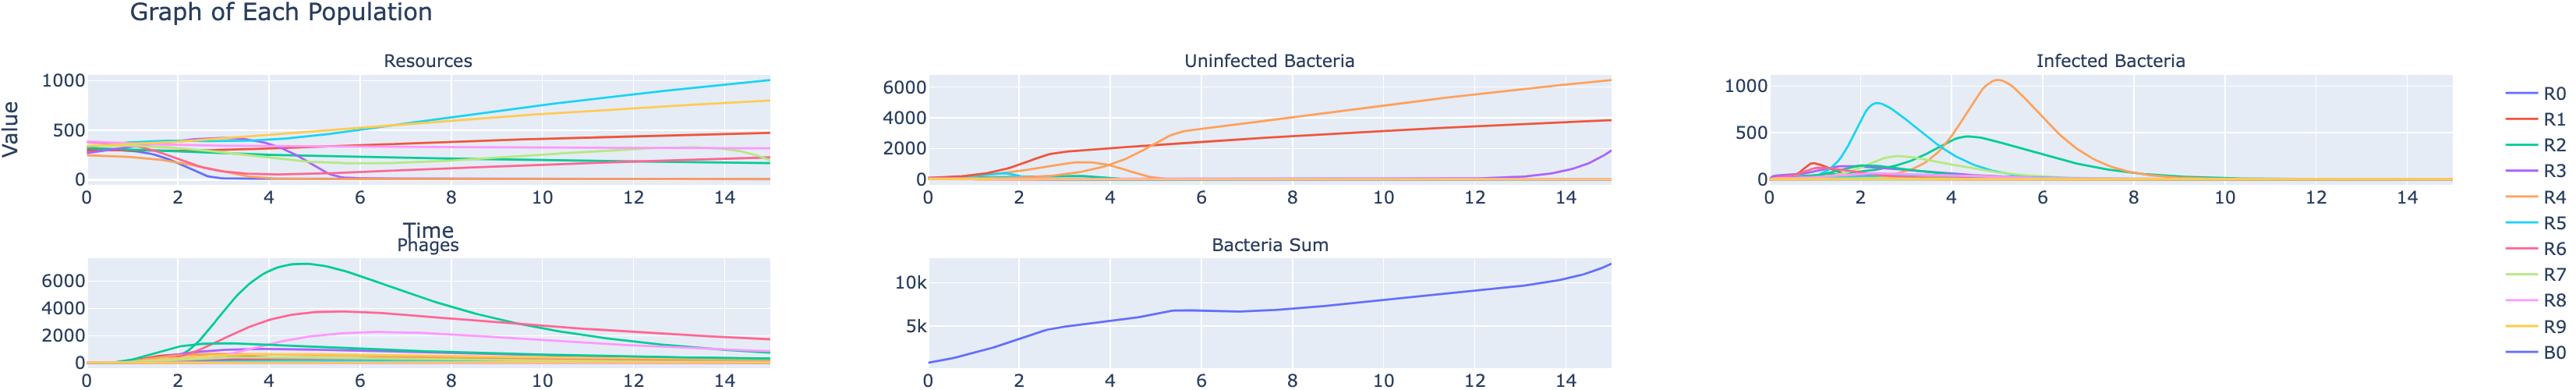
\includegraphics[width=\linewidth]{Plots/Created/debris.png}
        \caption{
            The $20\times20\times10$ model with a debris factor included. 
        }
        \label{fig:created:debris_model}
    \end{subfigure}
    \hfill
    \begin{subfigure}{1\linewidth}
        \centering
        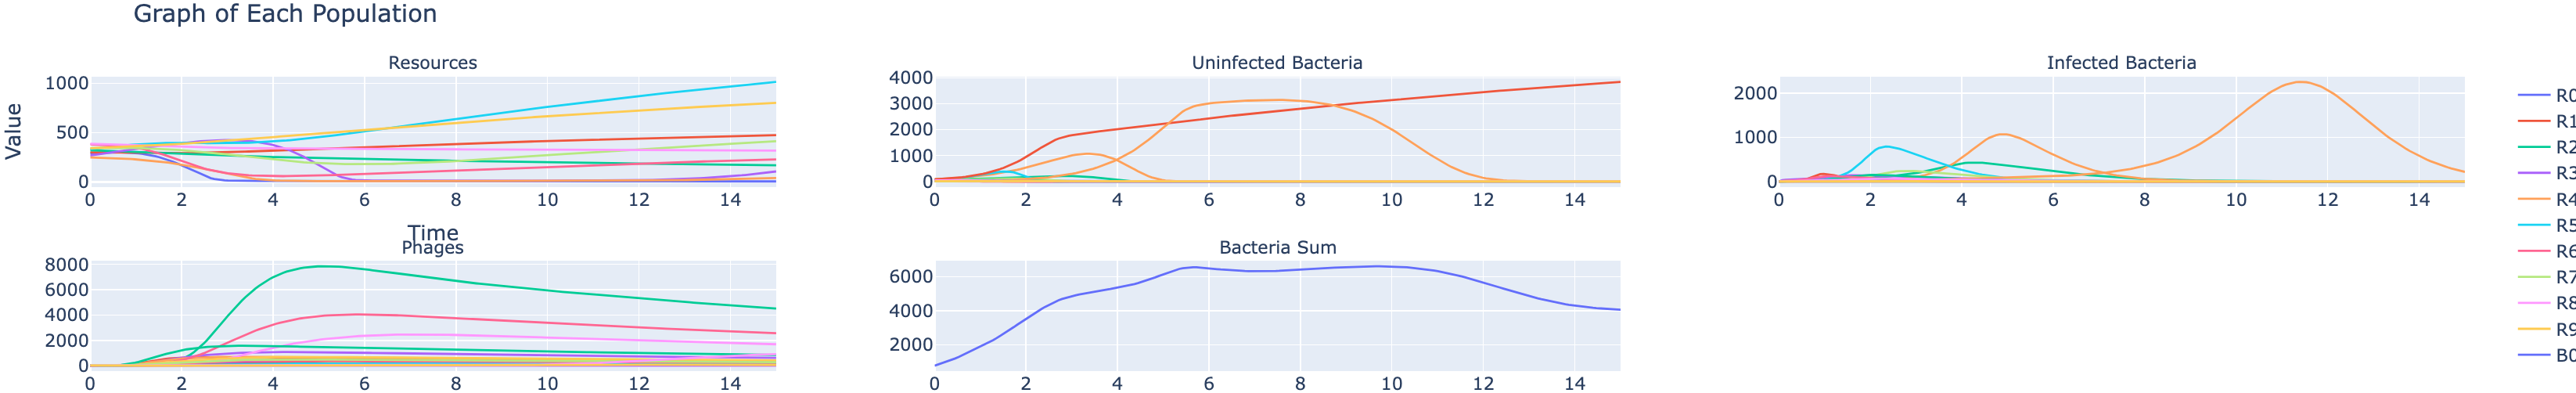
\includegraphics[width=\linewidth]{Plots/Created/no_debris.png}
        \caption{
            The $20\times20\times10$ model without the debris factor included. 
        }
        \label{fig:created:no_debris_model}
    \end{subfigure}
    \caption{
        A large $20\times20\times10$ model with a debris model added. 
        The debris parameter values were randomly and uniformly selected between 0.01 and 0.2.
    }
    \label{fig:created:debris}
\end{figure}